\documentclass[preprint,12pt,a4paper]{elsarticle}

\usepackage{amssymb}
\usepackage{booktabs}
\usepackage{graphicx}
\usepackage{hyperref}
\usepackage{lineno}
\usepackage{tabularx}
\usepackage{xurl}
\setlength{\parindent}{0pt}
\journal{SoftwareX}

\begin{document}
\begin{frontmatter}

\title{SeraEdit: Reliable Language-Guided MusicXML Editing through Structured Score Patches}

\author[aff1]{Yuan Gao\corref{cor1}}
\ead{[SUPPORT EMAIL]}
\ead[url]{https://orcid.org/0009-0005-0394-3623}
\cortext[cor1]{Corresponding author}
\address[aff1]{Zhejiang Conservatory of Music, No. 1 Zheyin Road, Zhuantang Street, Xihu District, Hangzhou, Zhejiang Province, China 310024}

\begin{abstract}
SeraEdit is local-first research software for reliable language-guided editing of
symbolic scores. Rather than asking a language model to rewrite an entire MusicXML
document, it represents a request as a versioned ScorePatch bound to stable event
identifiers, target and protected scopes, and a source fingerprint. Layered validators
check schema, score structure, duration, notation relations, protected content, and
MusicXML round-trip fidelity inside an atomic transaction. A desktop interface and
MuseScore bridge expose proposals, diffs, rejection reasons, and undo without silently
overwriting the host score. The release includes synthetic scores, editing tasks, three
evaluation conditions, resumable experiment tooling, and offline verification fixtures.
\end{abstract}

\begin{keyword}
MusicXML \sep symbolic music \sep score editing \sep structured patches \sep validation \sep research software
\end{keyword}
\end{frontmatter}

\begin{table}[!ht]
\small
\begin{tabularx}{\textwidth}{@{}l p{0.29\textwidth} X@{}}
\toprule
Nr. & Code metadata description & Metadata \\
\midrule
C1 & Current code version & \texttt{1.0.0-dev.14} \\
C2 & Permanent repository link & \url{https://github.com/Selancee/Sera}; must be public and tagged before submission \\
C3 & Reproducible capsule & [ZENODO OR CODE OCEAN DOI/URL] \\
C4 & Legal code license & MIT; benchmark data CC0-1.0 \\
C5 & Versioning system & Git \\
C6 & Languages, tools and services & Python, TypeScript/JavaScript, React, FastAPI, Electron, QML, PowerShell, MusicXML \\
C7 & Build, environment and dependencies & Python $\geq$3.10; Node.js/npm for interface development; Windows 10/11 desktop; requirements, tested Windows constraints and npm lock files \\
C8 & Developer documentation/manual & \texttt{docs/softwarex/}, reviewer guide and generated OpenAPI at \texttt{/docs} \\
C9 & Support email & [SUPPORT EMAIL] \\
\bottomrule
\end{tabularx}
\caption{Code metadata (mandatory).}
\label{tab:code-metadata}
\end{table}

\begin{table}[!ht]
\small
\begin{tabularx}{\textwidth}{@{}l p{0.29\textwidth} X@{}}
\toprule
Nr. & Executable software metadata description & Metadata \\
\midrule
S1 & Current version & \texttt{1.0.0-dev.14} \\
S2 & Permanent executable link & [RELEASE ASSET URL] \\
S3 & Reproducible capsule & [ZENODO OR CODE OCEAN DOI/URL] \\
S4 & Legal software license & MIT \\
S5 & Platforms & Windows 10/11 x64; source-level core uses Python $\geq$3.10 \\
S6 & Installation requirements & \texttt{docs/softwarex/INSTALLATION.md} \\
S7 & User manual & \texttt{docs/softwarex/USER\_MANUAL.md} \\
S8 & Support email & [SUPPORT EMAIL] \\
\bottomrule
\end{tabularx}
\caption{Executable software metadata (optional).}
\label{tab:software-metadata}
\end{table}

\linenumbers

\section{Motivation and significance}

MusicXML is a widely used interchange representation for common Western music
notation, allowing scores to move among notation, analysis, engraving, and archival
systems \cite{good2021musicxml}. Natural-language interfaces could reduce the
mechanical cost of local edits such as transposition, dynamics, articulation, or voice
assignment. However, asking a model to return a complete rewritten MusicXML document
mixes the intended change with thousands of unrelated elements. A syntactically valid
response can still alter an unselected staff, break a tie, change measure duration, or
drift from the source the user reviewed.

Symbolic-music toolkits provide programmatic analysis and generation
\cite{cuthbert2010music21,raffel2014prettymidi}, while recent work studies music
reasoning and generation with language models \cite{yuan2024chatmusician,zhou2024reason}.
SeraEdit addresses a narrower systems problem: making a language-guided edit
inspectable, source-bound, minimal, and rejectable before it returns to a professional
notation environment. The research object is therefore a transaction over a canonical
score representation, not an automatically accepted generated score.

The software supports controlled research on constrained generation, deterministic
evaluation of editing agents, repair/refusal policies, and human-in-the-loop notation
workflows. Three separately implemented conditions compare full-document rewriting,
unprotected structured patches, and a fully validated transaction without changing
source scores or metric code. This resembles structured code-editing evaluation
\cite{guo2024codeeditorbench}, but adds musical-time, voice, and notation-relation
invariants. Citation metadata follows software-citation principles
\cite{smith2016softwarecitation}.

\section{Software description}

\subsection{Software architecture}

Figure~\ref{fig:architecture} shows the local pipeline. A MusicXML snapshot is imported
into one canonical \texttt{ScoreDocument}. Editable events receive stable identifiers,
and a canonical SHA-256 fingerprint identifies the exact source state. Rendering,
preview, patch execution, MIDI conversion, and export consume the same document.

\begin{figure}[!ht]
\centering
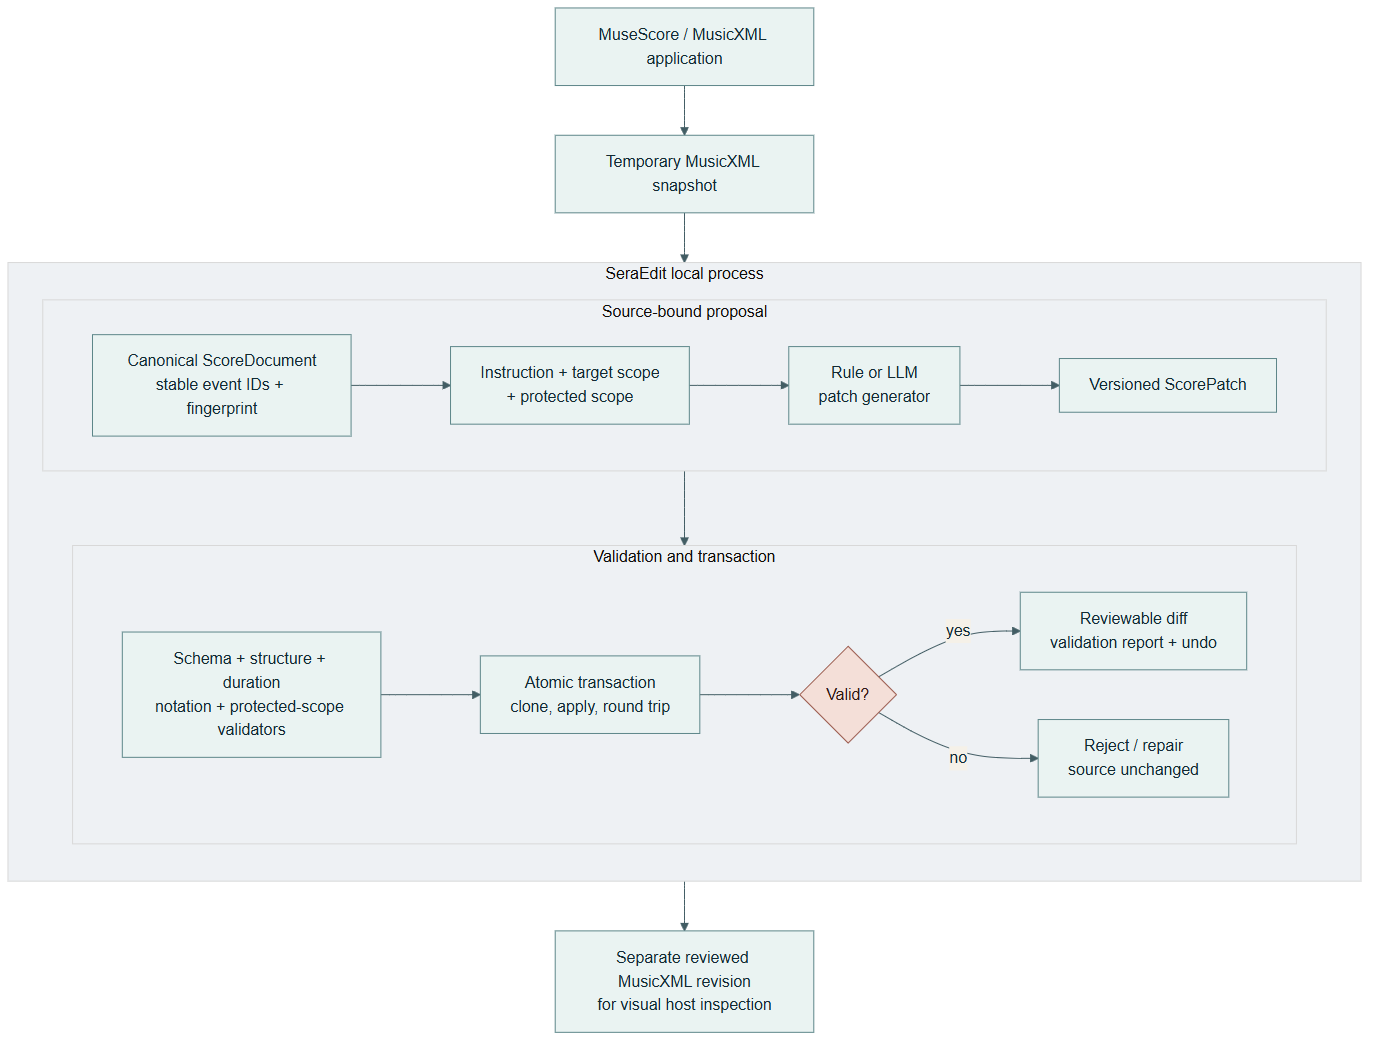
\includegraphics[width=\textwidth]{../figures/figure1_architecture.png}
\caption{SeraEdit component and transaction architecture. The notation host remains
the visual source. SeraEdit produces a separate reviewed revision or rejects the
transaction while retaining the source.}
\label{fig:architecture}
\end{figure}

Applying a patch validates the source fingerprint and schema, resolves selectors and
preconditions, clones the score, applies operations, validates the result, exports and
re-imports MusicXML, and finally commits or rolls back. The result contains normalized
errors, a human-readable diff, fingerprints, and snapshots for undo/redo. A transaction
failure cannot leave a partially modified score.

\subsection{Software functionalities}

A \texttt{ScoreScope} selects measures, parts, staves, voices, event identifiers, and
optional time ranges. Every patch declares editable and protected regions. Operations
use a versioned JSON schema and include selectors, arguments, preconditions, and
expected change counts. The research schema supports pitch and duration changes,
insertions and deletions, dynamics, articulations, ties, slurs, signature changes, voice
moves, motif duplication, chord replacement, and transactional batches. The product
enables only operation families with an established host round-trip contract; unknown
operations fail closed.

Validators cover schema, structural references, exact measure duration, notation
relations, semantic constraints, protected content, and MusicXML round trips.
Deterministic repair is restricted to transparent serialization corrections. Optional
model repair is bounded and receives immutable scopes plus explicit errors; it cannot
bypass the transaction.

Provider adapters record model, latency, token usage, estimated cost, request identifier,
finish reason, raw output, parsed output, and normalized errors. Secrets stay outside
source and experiment artifacts. The desktop can return local candidates before an
optional asynchronous model refinement completes. Neither path auto-applies a result.

The evaluation subsystem contains Full Rewrite, Patch Only, and Sera Full conditions.
Runs preserve configuration, prompt, benchmark and
dependency hashes, request caches, raw/normalized outputs, metrics, error records, and
resume state. Metrics are recomputed without another provider call.

\section{Illustrative examples}

For “Transpose measures 1--2 of staff 1 up two semitones and preserve rhythm; leave
staff 2 unchanged,” SeraEdit binds the proposal to the imported fingerprint and resolves
only pitched events in the requested region. Preview applies the transposition to a
clone. Duration equality is checked with rational values, protected staff 2 is compared
event-by-event, and exported MusicXML must parse, import, export, and parse again. A
valid preview reports the exact changed count; stale fingerprints, missing events,
duration changes, or protected differences reject and roll back the patch.

The optional MuseScore Studio 4 bridge exports a temporary snapshot and selection to
the local Sera process. After review, it opens a separate revised file. This is not
in-place control of MuseScore's internal document: the original open score is not
overwritten and final visual inspection remains a user action.

The offline core split contains 120 tasks over 20 short CC0 synthetic scores, spanning
pitch, rhythm, key and harmony, voice and texture, dynamics, insertion and deletion, relations,
meter, compound edits, and expected refusals. Each task declares target/protected scope
and deterministic constraints. The fixture provider returns known outputs to exercise
all runner and metric paths without network access or token cost.

For review, \texttt{scripts/run\_reviewer\_demo.py} runs six representative tasks
through the actual local product entry point and writes a compact report plus five
host-openable MusicXML revisions (the sixth task is an expected refusal). It needs no
API key or network connection. The included Windows CI workflow repeats the Python
tests, benchmark validation, reviewer demo, package audit, frontend tests, and build.

On Windows 11 build 10.0.26200 with Python 3.12.5, Node.js 24.16.0 and npm 11.13.0,
automatic benchmark validation accepted 120/120 task definitions. Human inspection
completed 120/120 current primary decisions and a stratified 30/30 repeat check with
zero stale records; all current decisions were compliant after correction. The
append-only export retains 194 records, including superseded findings. Both passes used
the same pseudonymous reviewer, so this verifies task/Gold semantics and host-visible
notation but not inter-rater reliability. The Python suite passed 408 tests.
Vitest passed 120 tests in 72 files; the Vite production build transformed 216 modules; and staged
backend, compatibility-launcher and Electron runtime smoke tests passed. A fresh
\texttt{softwarex\_verification\_120\_v1} fixture run completed 360/360 task-condition
cases with zero execution errors. Reproducibility checks confirmed configuration,
benchmark, prompt, dependency, evidence, metric-row and run-count integrity. These are
software verification results, not model performance: the manifest explicitly sets
\texttt{formal\_results\_allowed=false}.

We also replayed every instruction through the interactive product entry point without
supplying its Gold patch to generation. Across English and Chinese instructions and
three independent repetitions, 720/720 runs completed generation or expected refusal,
transaction preview, atomic commit, protected-scope checks, deterministic constraints,
and MusicXML export/re-import. All 660 executable runs produced valid MusicXML; 60
conflict runs refused safely; no unsafe execution occurred. Patch and result fingerprints
were identical in all 240 repeated task-language groups. After correcting a Chinese
preserve-pitch/tenuto ambiguity exposed by cross-language comparison, all 120 task groups
also produced semantically equivalent patches and identical English/Chinese final score
fingerprints. The compact snapshot preserves
all metrics and hashes for all 1,380 raw and host evidence files plus 220 host-openable
outputs for complete task review. This is
deterministic product-path acceptance, not remote-model accuracy or human musical quality.

We separately tested localization when the notation host supplied a wider selection
than the measure named in the instruction. The robustness runner added one adjacent
measure to each eligible explicit-measure request. It passed 240/240 bilingual runs;
expansion was applicable in 174 runs, and all 174 retained the intended task result,
protected content, and valid MusicXML. The remaining 66 tasks were not widened because
the instruction did not name a specific measure, the source lacked an adjacent measure,
or the operation was global. This is deterministic product evidence, not model accuracy.

\begin{table}[!ht]
\footnotesize
\begin{tabularx}{\textwidth}{@{}l r X X@{}}
\toprule
Evidence & Scale & Verified result & Claim boundary \\
\midrule
Benchmark & 120 tasks & 120/120 valid & Schema, Gold, constraints, round trip \\
Regression & 408 Python; 120 UI & All passed & Tested software environment \\
Reviewer demo & 6 tasks & 6/6; five host files & Offline product path \\
Product replay & 720 runs & 720/720; 660 exports & Local rules, not LLM accuracy \\
Host scope & 240 runs & 240/240; 174 widened & Target localization \\
Human review & 120 + 30 & Complete; zero stale & Same reviewer; no aesthetic claim \\
\bottomrule
\end{tabularx}
\caption{Triangulated release evidence and the boundary of each claim.}
\label{tab:evidence}
\end{table}

\section{Impact}

SeraEdit turns failure into inspectable research data. Rejections are classified by
stage, including malformed patches, invalid selectors, duration mismatches, broken
relations, protected-scope violations, incomplete execution, over-editing, conflicts,
unsupported operations, and provider timeouts. Raw outputs and deterministic metrics
enable studies of which safeguards affect validity, task completion, preservation,
minimality, repair, and refusal.

Researchers can add public-domain scores and task constraints without rebuilding a
front end, provider wrapper, transaction engine, or reporting pipeline. The offline
path supports continuous integration, teaching, and reproducibility; model-backed
runs remain clearly labeled. A desktop and MusicXML bridge expose the same contracts
to composers and notation users.

The source-bound scope/transaction pattern may also transfer to language-guided edits
of other structured scientific documents. Within music it supplies a foundation for
human studies without treating generated output as ground truth. Current evidence
supports reliability engineering and human-checked benchmark semantics, not aesthetic
improvement. Fixtures are small and synthetic, and the repeat check used the same
reviewer rather than an independent panel. Complex tuplets, grace relations, cross-voice
notation, and universal host compatibility are not established. MuseScore has an
exercised bridge; Sibelius is not claimed as verified. Provider behavior changes with
models and networks, while structural orchestration and unrestricted composition remain
outside the host-safe contract.

\section{Conclusions}

SeraEdit packages language-guided MusicXML editing as a source-bound, scoped, validated,
and reversible transaction. Models may propose, but canonical score state,
deterministic validators, protected-scope comparison, round trips, and user review
decide whether a revision exists. The open-source release candidate includes a desktop
demonstration, host bridge, benchmark, three conditions, automated metrics, tests, and
reproducibility tooling. Future work prioritizes formal model comparisons, cross-host
tests, richer notation relations, and independent blinded musician evaluation rather
than weakening the safeguards.

\section*{Author contributions}
Yuan Gao: Conceptualization, Methodology, Software, Validation, Investigation,
Data curation, Writing -- original draft, Writing -- review \& editing, Visualization.

\section*{Funding}
This research did not receive any specific grant from funding agencies in the public,
commercial, or not-for-profit sectors.

\section*{Declaration of competing interest}
[INSERT THE AUTHORS' VERIFIED DECLARATION.]

\section*{Data and code availability}
Source, CC0 benchmark fixtures, and the non-formal verification run will be available
from the tagged public repository and permanent archive in Table~\ref{tab:code-metadata}.
No API key or user score is distributed.

\begin{thebibliography}{00}
\bibitem{good2021musicxml}
M. Good (Ed.), MusicXML 4.0, W3C Music Notation Community Group Final Report, 2021.
\newblock \url{https://www.w3.org/2021/06/musicxml40/}.

\bibitem{cuthbert2010music21}
M. S. Cuthbert, C. Ariza, music21: A toolkit for computer-aided musicology and
symbolic music data, in: Proceedings of ISMIR, 2010, pp. 637--642.

\bibitem{raffel2014prettymidi}
C. Raffel, D. P. W. Ellis, Intuitive analysis, creation and manipulation of MIDI
data with pretty\_midi, in: ISMIR Late-Breaking and Demo Papers, 2014.

\bibitem{yuan2024chatmusician}
R. Yuan et al., ChatMusician: Understanding and generating music intrinsically with
LLM, in: Findings of ACL, 2024.

\bibitem{zhou2024reason}
Z. Zhou et al., Can LLMs ``reason'' in music? An evaluation of LLMs' capability of
music understanding and generation, in: Proceedings of ISMIR, 2024.

\bibitem{guo2024codeeditorbench}
J. Guo et al., CodeEditorBench: Evaluating code editing capability of large language
models, arXiv:2404.03543 (2024).

\bibitem{smith2016softwarecitation}
A. M. Smith, D. S. Katz, K. E. Niemeyer, FORCE11 Software Citation Working Group,
Software citation principles, PeerJ Computer Science 2 (2016) e86.
\newblock \url{https://doi.org/10.7717/peerj-cs.86}.
\end{thebibliography}

\end{document}
